\documentclass{article}
\usepackage[utf8]{inputenc}
\usepackage{morefloats}

\title{Astronomy 121 Lab 3: Radio Interferometry at X Band}
\author{Vikram Iyer}
\date{\today}

\usepackage{natbib}
\usepackage{graphicx}
\usepackage{listings}
\usepackage{placeins}
\usepackage[margin=1.0in]{geometry}


\begin{document}

\maketitle

%=======================================================================================

\begin{abstract}
    This lab experiment focused on understanding and using a multiplying interferometer
    composed of 2 1m dishes observing at X band separated by 10m along an approximately East-West
    baseline on the roof of Wurster Hall at UC Berkeley (37.8732, -122.2573) to
    observe the sun, moon, and various point sources. A least squares regression was
    used to approximate a function to fit the data and thereby determine an
    exact value for the baseline length using known catalog values for the
    declination of the source. Analysis of the strongest frequency components in
    the data from 3C144 (the Crab Nebula) showed the baseline distance to be
    8.352m. A separate analysis with a very narrow bandwidth filter in what
    appears to be noise in the original spectrum yields a baseline value of
    10.016m. A similar procedure was used to analyze the sun and moon data to
    determine their fringe frequency and thereby determine their radius by
    comparing the fringe frequency to an ideal Bessel function representing the
    intensity of these sources. The diameter of the sun was calculated to be
    $0.4312^{\circ}$ and
    the diameter of the moon was determined to be $D = 0.34844^{\circ}$. This
    analysis used the assumed baseline distance of 10m rather than the value
    calculated from the analysis of the point source. Calculations of the cable
    delay from all analyses were inconclusive.
\end{abstract}

%=======================================================================================
%Need

\section{Introduction}
Interferometry is a common tool in radio astronomy both for the purpose of
correlating multiple signals to improve the signal to noise ratio (SNR)
of weak astronomical signals, as well as to improve the resolution with which
one can observe the sky. The purpose of this lab experiment was to learn and
apply the basic principles of interferometry to measure the diameter of the sun
and the moon, as well as the baseline length of the interferometer from the
known declination of a point source. After recording and processing the raw data
we applied least squares to obtain a function of best fit to the processed data in order to determine the quantities of interest such as source diameter and
baseline.
%=======================================================================================
%citep
\section{Methods}
  \subsection{Interferometer}
  We began this lab experiment by learning about the basics of interferometry as
  well as the details of the system we used for collecting data.

  \subsubsection{A Two Element Interferometer}
  A two-element interferometer consists of two telescopes separated by some
  baseline vector $\vec{b}$. Both telescopes receive radiation from the observed
  source and these signals are multiplied together to form the output. Because
  of the separation of the two telescopes, there is a delay between the time at
  which waves from the source reach the first telescope and the second one.

  We can define the signals that each antenna detects as follows:
  \[E_{i}(t) = e_{1}(t) + e_{2}(t)\]
  \[E_{j}(t) = e_{1}(t-\tau_{1}) + e_{2}(t-\tau_{2})\]

  Correlating these received signals from the two antennas results in the
  average power received. The output of correlation should result in a set of
  values in the power spectrum which are significantly larger than the noise.

  \subsubsection{Wurster Hall Interferometer}
  The interferometer consists of two 1m diameter dishes along an approximately
  10m East-West baseline located on the lower roof of Wurster Hall at UC
  Berkeley. Each antenna output is connected to a series of analog
  filters and amplifiers prior to sampling.  After initial amplification and
  filtering at the source of the signal, the inputs are down converted from an
  original frequency of 10.7 GHz. This output is down converted again and
  filtered to a bandwidth of 30MHz. The outputs of the two dishes are then mixed
  and sampled.  The data is collected by an HP digital voltmeter connected via
  GPIB to a Linux workstation. This computer is capable of both recording the
  output as well as controlling the motors to point the telescope. The full
  signal path is shown in \ref{fig:signal_path}.

    \begin{figure}[h!]
    \centering
    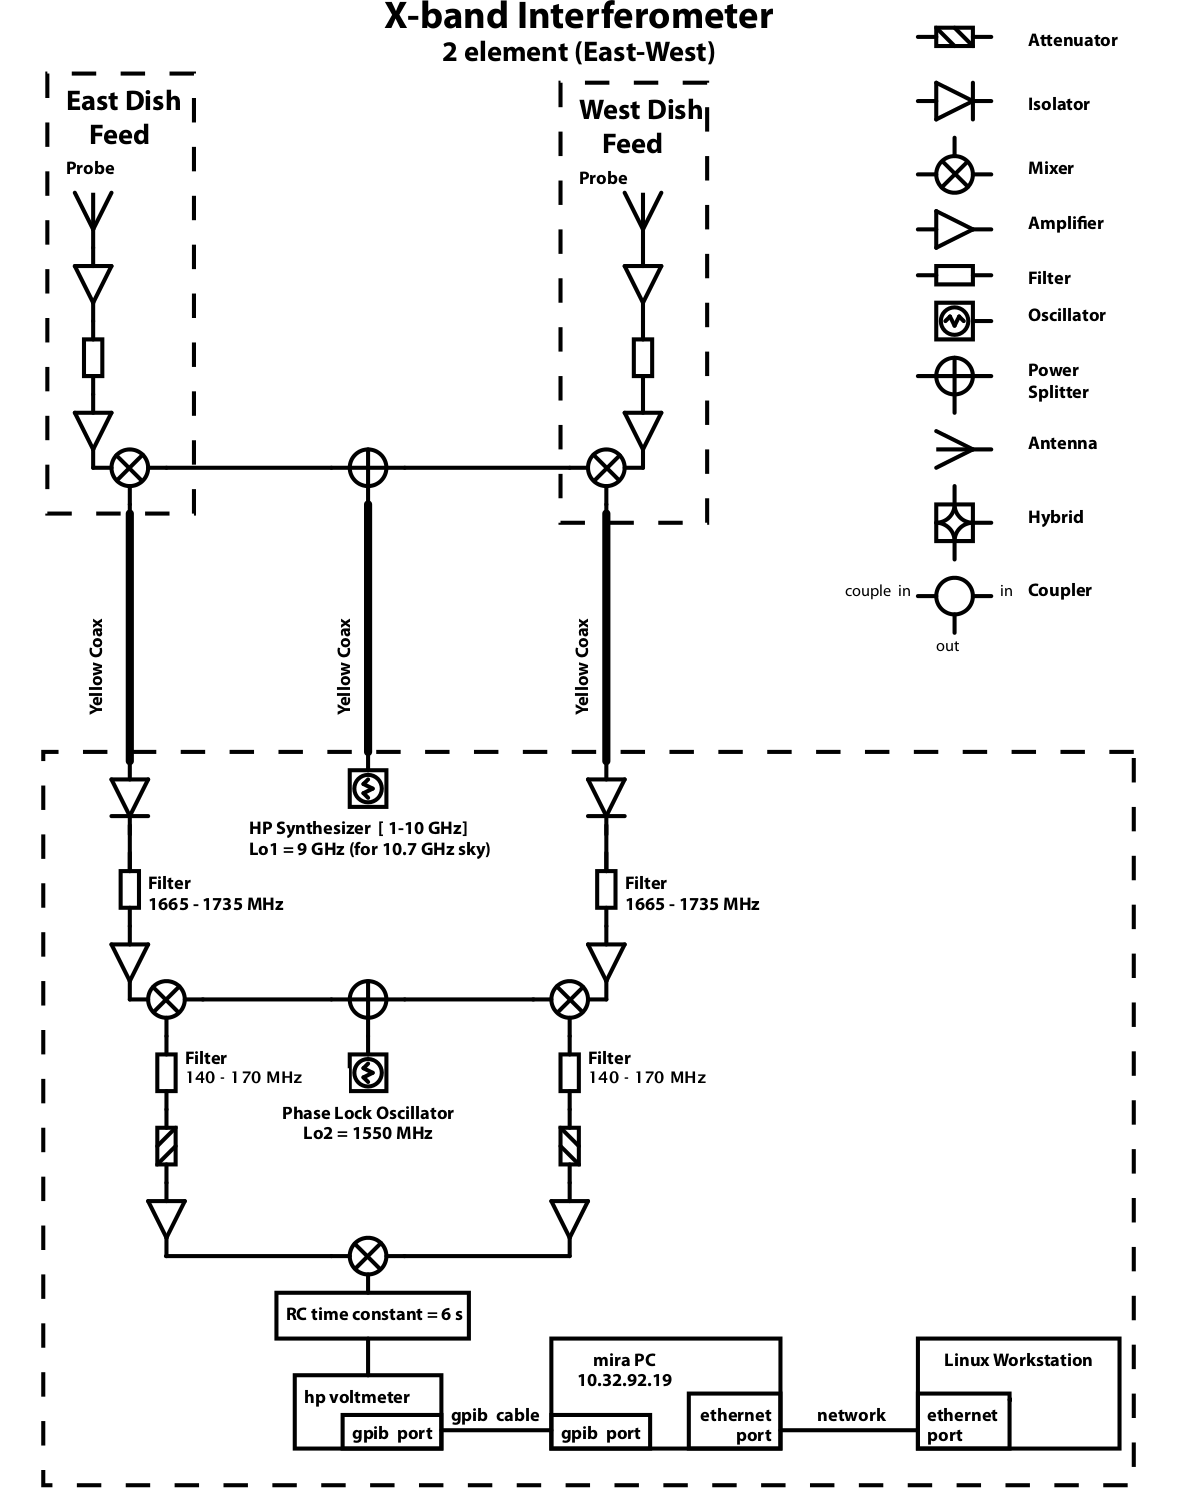
\includegraphics[scale=0.3]{img/signal_path.png}
    \caption{Block diagram of the interferometer on the roof of Wurster Hall.}
    \label{fig:signal_path}
    \end{figure}

  This interferometer is mechanically limited to an altitude range of
  $15^{\circ}$ to $87^{\circ}$. Additionally, tall buildings such as the
  Campanile and the other half of Wurster Hall further limit the
  interferometer's field of view. The interferometer can be pointed to a
  specified altitude and azimuth value within the range described, and can be
  updated less than every 30 seconds. The dishes' encoders do however
  accumulate error over time and must be reset to a home position every 2-3
  hours.

  \subsection{Coordinate Transformations}
  In order to accurately point the interferometer at sources, we had to
  calculate the positions of sources and update them in real time. The point
  sources of interest all had known known right ascension (RA) and declination
  (DEC) values, however we had to convert these to an altitude and azimuth in
  order to point the telescope.

  To perform the conversion we first converted the given coordinates from
  (RA, DEC) to (HA, DEC) by taking the dot product of the original coordinates
  as a vector with the following rotation matrices.

   \[ {R}_{(\alpha , \delta ) \rightarrow (ha, \delta )} =
      {R}_{(\alpha , \delta) \rightarrow (ha, \delta ),2} \cdot
      {R}_{(\alpha , \delta ) \rightarrow (ha, \delta ),1} \]

   \[ {R}_{(\alpha , \delta ) \rightarrow (ha, \delta ),1} = \\
       \left [ \begin{array}{ccc}
           \cos(LST) & \sin(LST) & 0 \\
           -\sin(LST) & \cos(LST) & 0 \\
           0 & 0 & 1 \\
       \end{array} \right ]  \]

   \[ {R}_{(\alpha , \delta ) \rightarrow (ha, \delta ),2} = \\
       \left [ \begin{array}{ccc}
           1 & 0 & 0 \\
           0 & -1 & 0 \\
           0 & 0 & 1 \\
       \end{array} \right ]  \]

  After converting the values to terms of HA, which is dependent on a
  terrestrial position, we converted from (HA, DEC) to (ALT, AZ) based on our
  latitude $\phi$ using the following matrix.
   \[ {R}_{(ha , \delta ) \rightarrow (az, alt)} = \\
       \left [ \begin{array}{ccc}
           -\sin(\phi) & 0 & \cos(\phi) \\
           0 & -1 & 0 \\
           \cos(\phi) & 0 & \sin(\phi) \\
       \end{array} \right ]  \]

  In order to accurately determine RA and DEC at the time of observation, we
  precessed the catalog values of RA and DEC for the epoch 2000. To perform this
  calculation we used the Python module PyEphem. In addition PyEphem
  contains useful options to calculate the altitude and azimuth of the sun and
  moon. This is particularly useful for the moon as it accounts for the effects
  of observing an object so close to the Earth. We also used the
  \lstinline{ephem.FixedBody} object to actually perform the calculation of
  the altitude and azimuth for the point sources when collecting data. The
  details of the implementation can be found in \lstinline{observe.py}.

  \subsection{Data Collection}
  As explained previously, the interferometer is connected to a Linux computer
  that is remotely accessible. In order to collect data, we had to ensure that
  the position of the interferometer was updated regularly to be directed at the
  source. Additionally we had to regularly reset the telescope to a reference
  position in order to prevent excessive accumulation of error from the
  encoders. We recalculated the position of the Sun and the Moon every 30
  seconds as their position changed more quickly over time, and every 60 seconds for
  the point sources.

  \subsubsection{Data Collection Script}
  In order to automate our data collection, we wrote a Python script to
  calculate the position of the observed source at a given frequency as well as
  collect and save the data from the digital voltmeter (DVM). The script itself is
  divided into two main functions that run in separate threads; the first of
  these functions \lstinline{controller} calculates the position of the source
  every \lstinline{t} seconds and re-points the telescope while the
  \lstinline{recordData} function records data from the DVM and saves the output
  to a specified file. The source position updates were calculated based on
  updating the time of the \lstinline{ephem.Observer} object used by PyEphem to
  compute the altitude and azimuth. As shown above, while our location on Earth
  was fixed, converting (RA,DEC) to (ALT, AZ) at a specific location requires
  the local sidereal time (LST) which we obtained using the
  \lstinline{ephem.now} function.

  Both the data record data and controller were run in separate threads so that
  we could record data continuously rather than having to pause and resume data
  collection to re-point the telescope every 30 seconds. In addition both
  threads were run as daemons to ensure consistency in the data (ie to account
  for cases in which the pointing may have failed, at which point recording data
  additional data would have been misleading). All functions used Python's
  logging utility to record detailed debug and warning messages for reference
  during data analysis. The full data collection script is available with
  detailed function documentation in \lstinline{observe.py}.

  \subsubsection{Observed Sources}
  We observed a variety of sources including the Sun from horizon to horizon, as
  well as the Moon and point sources such as 3C144 (the Crab Nebula). We began
  by observing the Sun for a period of 1 hour, mainly to ensure that our data
  collection script was properly tracking and recording sources. After this we
  observed the Sun from horizon to horizon to gather data necessary for
  determining its diameter. We attempted to observe the moon multiple times,
  however most of these observations were within a few days of a new moon at
  which point only 15\% of the moon was actually illuminated. We obtained
  an additional observation of the moon for 4 hours approximately a week after
  the new moon at which point 30\% was illuminated. We attempted to observe
  multiple point sources including Orion, the Crab Nebula, and M17 as well.

  \subsection{Data Processing}
  Although the interferometer does correlate the signals received from the two
  telescopes, the radiation from most astronomical sources is negligible
  compared to other sources of electromagnetic radiation. while we were able to
  identify peaks corresponding to each source, the SNR was relatively low for
  all of the sources other than the sun. In order to process the data and
  calculate the values of interest, we attempted a variety of filtering
  techniques.

  \subsubsection{Point Souce Data}
  In order to isolate the frequencies corresponding to the point source, we
  attempted to filter the data in a variety of ways. These included a median
  filter to smooth the data, as well as band pass filters of varying bandwidth,
  windowing functions, and numbers of coefficients. We also attempted zeroing
  out entire ranges of values in the frequency domain and taking the inverse
  Fourier transform.

  The general method we used for processing the point source data consisted of
  attempting to visually identify peaks corresponding to what were likely
  frequencies from the observed source. We also experimented with a few other
  ideas such as attempting to normalize the signal over a range of values, as
  the expected signal should have been roughly a constant amplitude. We also
  attempted analyzing subsections of the datasets for those in with some kind of
  unexpected behavior in the time domain.

  \subsubsection{Least Squares Fitting}
  After filtering the raw data, we applied least squares to fit a known model
  of the source to the measured values to determine the unknown parameters.

  Ordinary least squares (OLS) corresponds to solving a simple optimization
  problem of the form

  \[\min{x} ||Ax - y||^2_2 \]

  This model is useful for estimating solutions to problems for which $Ax=y$ is
  not feasible. We there for project $y$ onto $Ax$ and attempt to minimize the
  squared Euclidean distance between them. The closed form solution to this
  problem is:

  \[x* = (A^{T}A)^{-1}A^{T}y \]

  In order to solve for the parameters corresponding to the equation for the
  interferometer output, we applied least squares.  Although this model is
  nonlinear we assumed the function to be roughly linear considering $\sin(h_s)$
  increases monotonically over time for a range of values.

  \[F(h_{s} = A\cos \left [C\sin(h_{s})\right] - B\sin \left
  [C\sin(h_{s})\right]\\
  C = \frac{B_{y}}{\lambda}\cos(\delta)
  \]

  We began by determining the known precessed declination of the source and
  assuming the wavelength $\lambda = 2.5cm$. To solve for the baseline $B_{y}$,
  we iterated over 500 values in the range of 700cm to 1200cm. For each value we
  saved the residuals, and chose the value corresponding to the minimum residual
  value as the optimal or \"true\" baseline length. We then used the
  coefficients from this regression to estimate $\tau_c$, the cable delay.

  \subsubsection{Calculating diameter}
  We used similar signal processing techniques to filter the data for the Sun
  and the Moon. In the case of these data sets we attempted to preserve the
  envelope of the data, as it contains the information necessary to calculate
  radius.

  We used a similar method of applying least squares as for the point source to
  fit an equation of the following form:

  \[F(t) = \cos \left (2\pi \frac{B_{y}}{\lambda} \cos(\delta)
      sin(h_{s}) + \phi \right)\]

  We chose not to use the baseline and cable delay calculated previously as they
  were very inconsistent. We attempted fitting both to the filtered data itself as well as its envelope
  calculated by convolving the absolute value of the data with a low pass filter.
  After obtaining this function by iterating over guesses of $\phi$, just as
  solving when for $B_{y}$, we chose the corresponding value that minimized the
  error term.

  The goal of doing all of this was to fit a function to the data over a narrow
  region to find the points at which it crossed 0. The envelope of the Sun and
  the Moon signals are ideally Bessel functions, which are functions of  $R \cdot
  F_{f}$. By determining a fringe frequency $F_{f}$ corresponding to the zero
  crossing, we matched that $F_{f}$ to a value of $F_{f}$ on the $R \cdot
  F_{f}$ axis of the Bessel function.

  \[F_{f} = \left (\frac{B_{y}}{\lambda}\cos(\delta)\right ) \]

  To match the Bessel function with the envelope of the data, we used trial and
  error to shift it to a point which seemed to correspond to the measured data.
  Because the Bessel function crosses the x axis at integer values we can solve
  for the radius.

  \[RF_{f}=\frac{k}{2} \\
      R = \frac{k}{F_{f}} = \frac{\lambda}{B_{y}\cos(\delta)\cos(h_{s})}
  \]

  We then multiplied this value of the radius in degrees by 2 to determine the
  angular diameters of the sources in degrees.

%=======================================================================================

\section{Results \& Discussion}

\subsection{Point Source (3C144)}
  Figure \ref{fig:crab_raw} shows the raw data from observing 3C144 (the Crab
  Nebula) on 03/28/2014 beginning at 0:19:26 UTC. The power spectrum shows two
  peaks symmetric about zero that correspond to what we might expect to see as
  the output of the interferometer.

    \begin{figure}[h!]
    \centering
    \includegraphics[scale=0.5]{img/crab/raw.png}
    \caption{Raw data and power spectrum from the observation of 3C144 with the
    DC offset subtracted.}
    \label{fig:crab_raw}
    \end{figure}

  In order to isolate these peaks we first tested a variety of median filters.
  The result of applying median filters is shown in Figure
  \ref{fig:median_test}. This low pass filtering eliminated many of the high
  frequency components due to repointing. We chose a window of size 9 so as not
  to eliminate frequencies surrounding the peak that may have been important.

    \begin{figure}[h!]
    \centering
    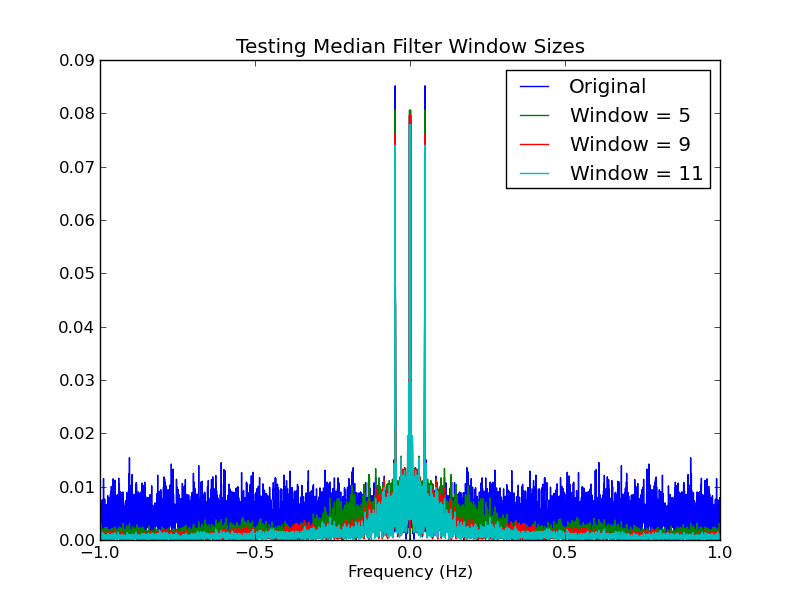
\includegraphics[scale=0.5]{img/crab/median_test.png}
    \caption{Effects of median filter with varying window sizes on the
    spectrum of the signal.}
    \label{fig:median_test}
    \end{figure}

  The data also appeared to have large irregularities in certain sections, of
  approximately 2000 seconds. This may have been due to other objects
  obstructing the telescope such as the other campus buildings mentioned
  previously. More likely however, these irregularities were probably caused by
  the repointing of the telescope as they occur both close to the beginning of
  the observation, as well as some point later in the observation. Interestingly
  the duration appears to be much longer than the time to run the homing
  procedure.
    In order to simplify the data processing we isolated a single
  segment of the raw data from 2000 to 6000 seconds (corresponding to the
  original observation. Figure \ref{fig:seg} shows a plot of this data and that
  the amplitude of the assumed peaks of interest are much larger in the power
  spectrum.
    \begin{figure}[h!]
    \centering
    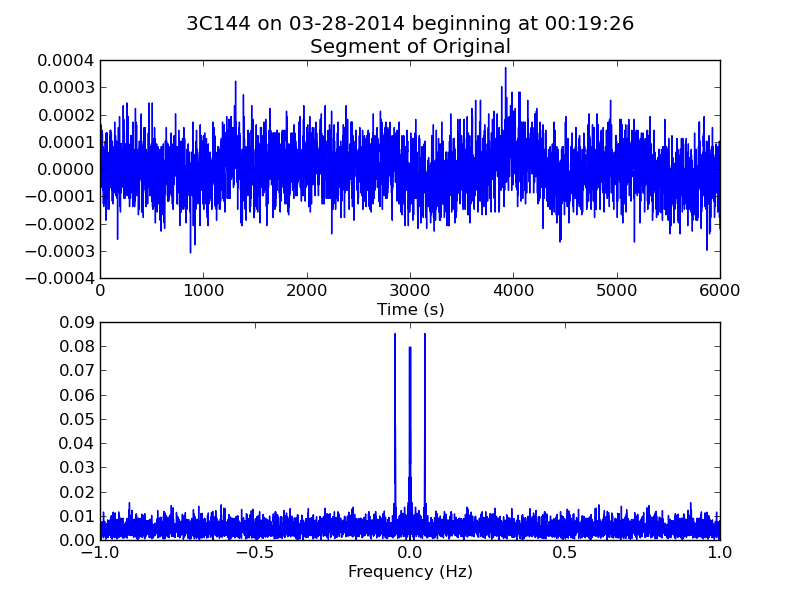
\includegraphics[scale=0.5]{img/crab/seg.png}
    \caption{Segment of the raw data in which the frequency components of
    interest appear to be significantly stronger.}
    \label{fig:seg}
    \end{figure}

  Continuing in the attempt to isolate the observed peaks, we next tested a
  series of FIR band pass filters to further isolate the peaks we noticed in the
  original spectrum. Figure \ref{fig:bandpass_test_d} shows the result of
  applying these filters. Based on this we chose a filter with 256 taps centered around 0.05 Hz
  with a bandwidth of 0.01.

    \begin{figure}[h!]
    \centering
    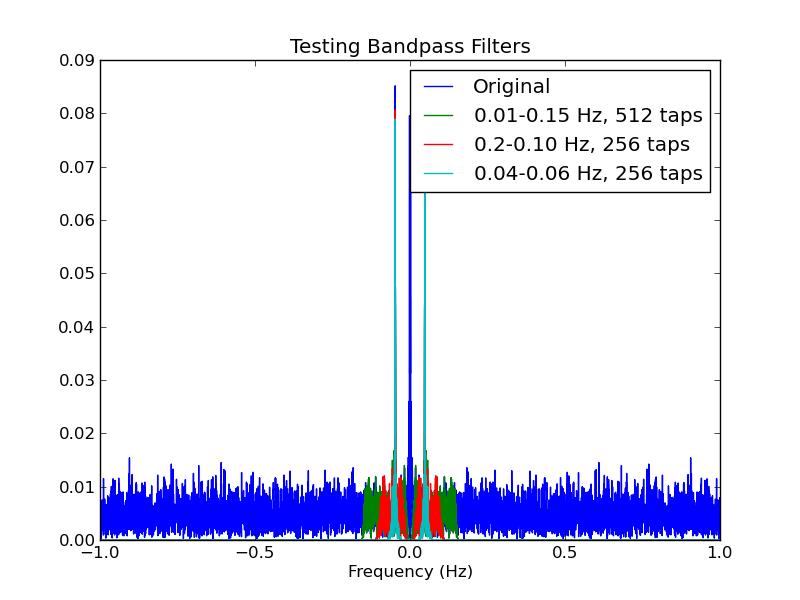
\includegraphics[scale=0.5]{img/crab/bandpass_test_d.png}
    \caption{Effects of band pass filters with various parameters on the
    spectrum of the selected segment of the signal.}
    \label{fig:bandpass_test_d}
    \end{figure}


    We also normalized the data to a range of -1 to 1 by dividing it by its
    maximum.  The resulting filtered and normalized signal is shown in Figure
    \ref{fig:baseline_filtered_seg}.

    \begin{figure}[h!]
    \centering
    \includegraphics[scale=0.5]{img/crab/baseline_filtered_seg.png}
    \caption{Result of filtering the selected segment of the signal to isolate
    the peaks visible in the unfiltered spectra.}
    \label{fig:baseline_filtered_seg}
    \end{figure}

    After filtering the signal we applied least squares as described previously
    to fit a function to this data. Figure \ref{fig:fit_baseline_seg} shows the
    result. This simple attempt to use linear least squares appears to have some
    visual relationship to the data.

    \begin{figure}[h!]
    \centering
    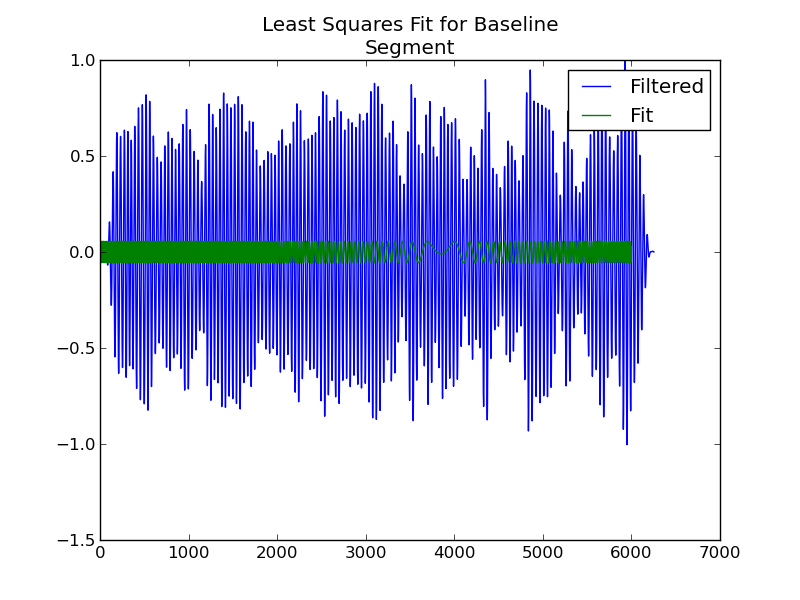
\includegraphics[scale=0.5]{img/crab/fit_baseline_seg.png}
    \caption{Result of least squares fitting to the filtered segment of the data.}
    \label{fig:fit_baseline_seg}
    \end{figure}

    Figure \ref{fig:residual_baseline_seg} shows the square of the residuals
    from applying least squares. The values are normalized to a maximum scale of
    1. There is a noticeable minimum in this plot, however it corresponds to a
    value significantly lower than the known baseline of approximately 10m, and
    the scale of the difference between these values does not appear to be
    significant (less than 1\%).

    \begin{figure}[h!]
    \centering
    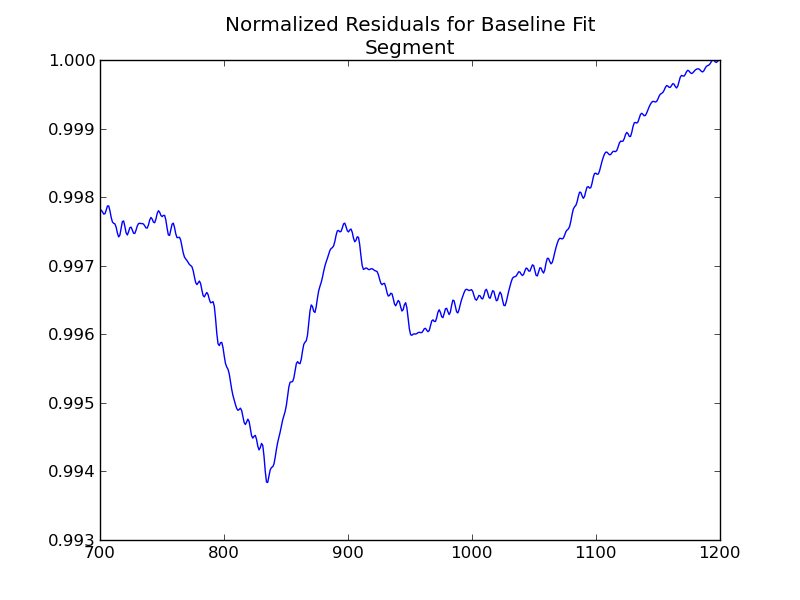
\includegraphics[scale=0.5]{img/crab/residual_baseline_seg.png}
    \caption{Residuals from fitting to the filtered segment of data.
    The residuals are plotted against the values of the baseline
tested ranging from 700cm to 1200cm}
    \label{fig:residual_baseline_seg}
    \end{figure}

    Considering the fringe frequency increases linearly with the baseline, we
    attempted to filter out other sections of the data to isolate a range that
    may include the actual fringe frequency. We chose values significantly
    higher than the peak visible in the original spectrum.  The original
    observed peak produced a fairly obvious minimum error when applying least
    squares, so we chose a different part of the spectrum in the event that the
    visible peaks were not actually the fringe frequency of interest.  The result of testing different
    band pass filters at higher frequencies is shown in Figure
    \ref{fig:bandpass_test_b}. We applied these filters to the original data set
    and ended up choosing an even narrower filter with a bandwidth of 0.005 Hz
    centered around 0.2 Hz.

    \begin{figure}[h!]
    \centering
    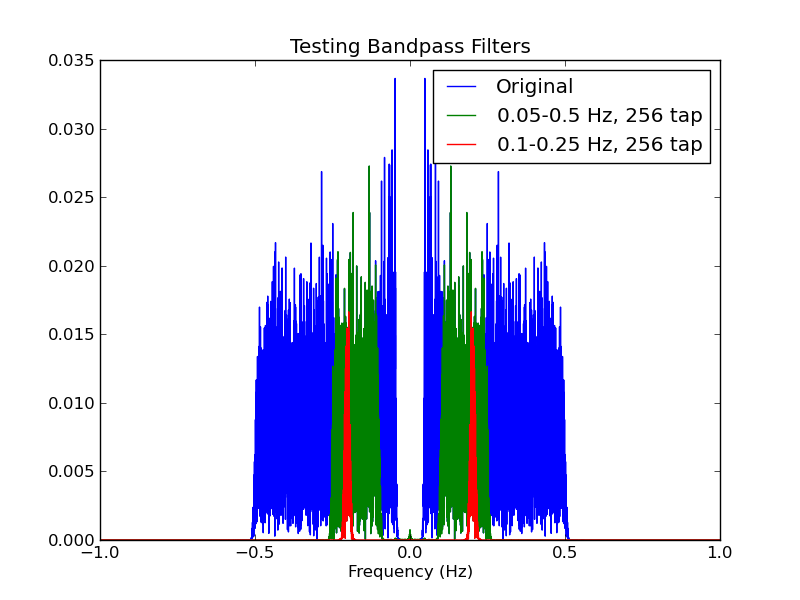
\includegraphics[scale=0.5]{img/crab/bandpass_test_b.png}
    \caption{Effect of applying narrow band pass filters centered at higher frequencies.}
    \label{fig:bandpass_test_b}
    \end{figure}

    The result of applying this filter is shown in Figure
    \ref{fig:baseline_filtered}.

    \begin{figure}[h!]
    \centering
    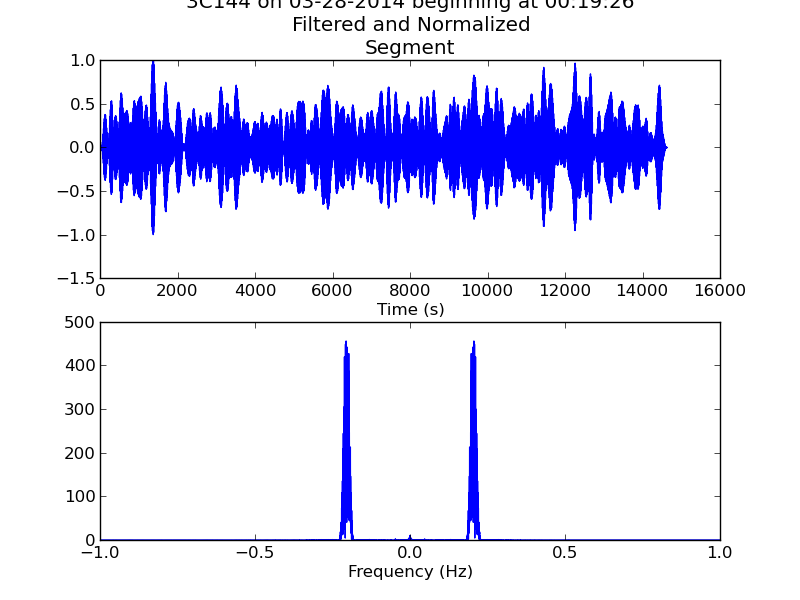
\includegraphics[scale=0.5]{img/crab/baseline_filtered.png}
    \caption{Result of applying a narrow band pass filter to isolate higher
    frequencies.}
    \label{fig:baseline_filtered}
    \end{figure}

    After filtering we attempted the same least squares analysis on this data.
    The result is shown in Figure \ref{fig:fit_baseline}.

    \begin{figure}[h!]
    \centering
    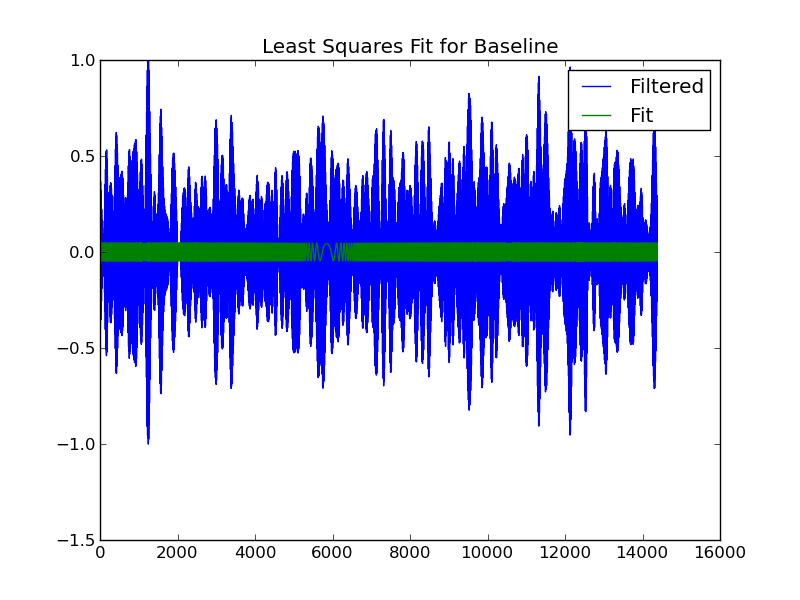
\includegraphics[scale=0.5]{img/crab/fit_baseline.png}
    \caption{Result of applying least squares to fit a narrow band of higher
    frequencies.}
    \label{fig:fit_baseline}
    \end{figure}

    Figure \ref{fig:residual_baseline} shows the residual from applying least
    squares to this very narrow band of frequencies. Interestingly the resulting
    minimum error is more significant than the previous one (a difference of 6\%
    between the most significant peaks compared to 0.2\% with the previous
    analysis). The resulting value is also very close to the expected baseline
    of 10m, however the plot of the residuals still appears to vary
    significantly and has other local minima. This may simply be due to our
    attempt to apply this analysis technique intended for linear or affine
    functions to this problem.  Although the hour angle does increase
    monotonically as explained in the lab document, $sin(h_{s})$ can only be
    approximated by a linear function for a certain range.

    \begin{figure}[h!]
    \centering
    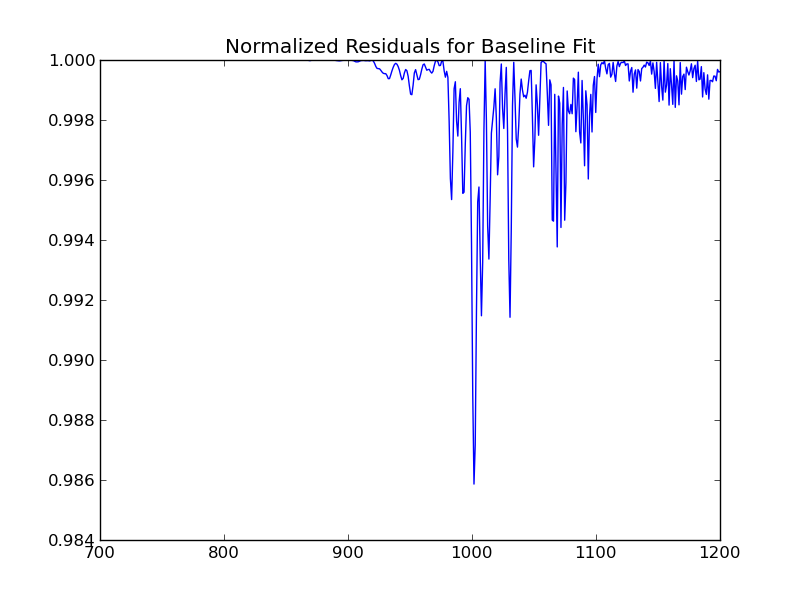
\includegraphics[scale=0.5]{img/crab/residual_baseline.png}
    \caption{Residuals from applying least squares to fit a narrow band of higher
    frequencies. The residuals are plotted against the values of the baseline
tested ranging from 700cm to 1200cm}
    \label{fig:residual_baseline}
    \end{figure}

    While we were able to determine a value of the baseline $B_y=1001.603cm$ close to the
    expected 10m, the fact that the range of frequencies we analyzed didn't
    correspond to the most noticeable peaks suggests the presence of some other strong
    source. We therefore applied the same least squares analysis to attempt to
    determine the of this source assuming a baseline length of 10m and varied
    $\cos(\delta)$ over a range of 0 to 90. We chose this range to eliminate the
    because we assumed the declination of the interfering source to be similar
    to that of 3C144, and because analyzing the full range of $\cos(\delta)$
    from -1 to 1 should produce roughly symmetric results. Figure \ref{fig:fit_dec} shows the result of this analysis.

    \begin{figure}[h!]
    \centering
    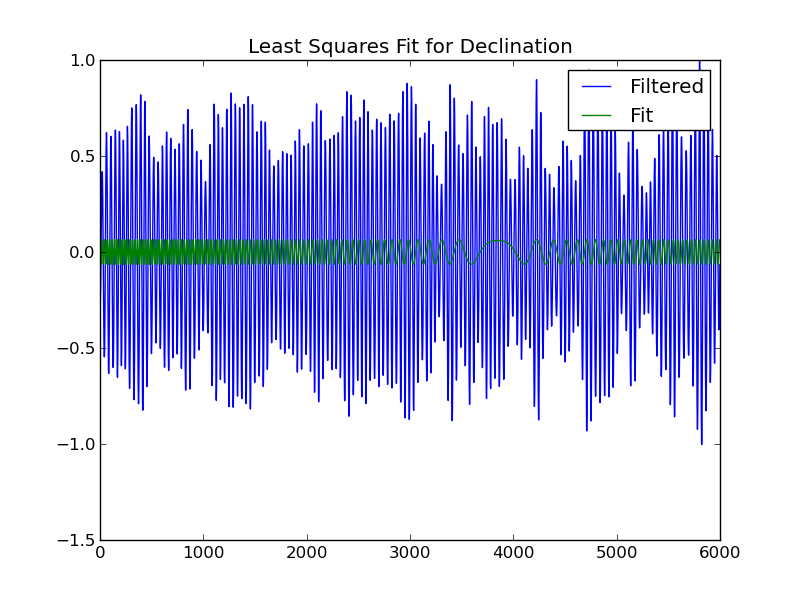
\includegraphics[scale=0.5]{img/crab/fit_dec.png}
    \caption{Result of applying least squares to fit a narrow band of higher
    frequencies.}
    \label{fig:fit_dec}
    \end{figure}

    When examining the residuals of this analysis in Figure
    \ref{fig:residual_dec}, we can see that there are numerous local minima
    that do not differ significantly. Based on this analysis the determined
    value of $\delta$ was $64.620\circ$.  The lack of any noticeable peak above the noise in the spectrum close to
    these frequencies suggests that we were just analyzing noise as the
    interferometer correlates the outputs of the two telescopes.

    \begin{figure}[htbp!]
    \centering
    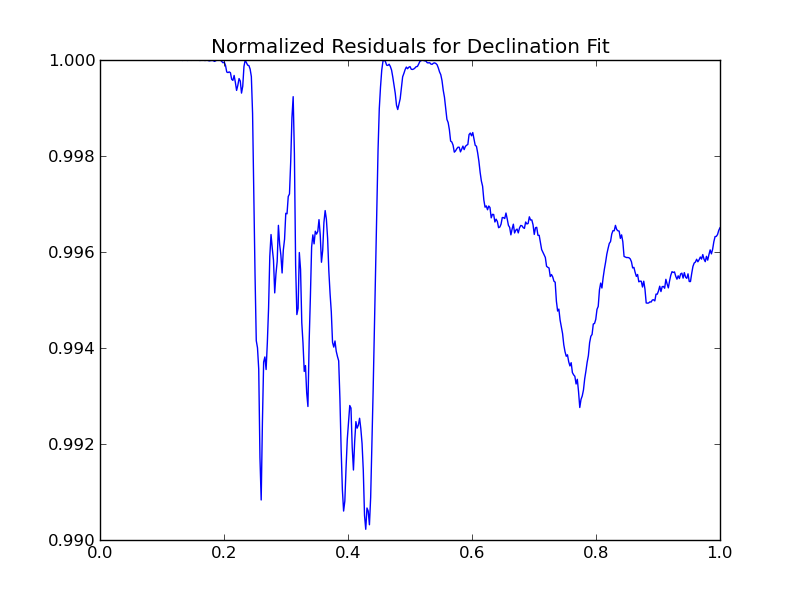
\includegraphics[scale=0.5]{img/crab/residual_dec.png}
    \caption{Residuals from applying least squares to fit a narrow band of higher
    frequencies. The residuals are plotted against the values of the
$\cos(\delta)$ from 0 to 1.}
    \label{fig:residual_dec}
    \end{figure}

    Based on the coefficients from our least squares approximations we can also
    calculate the cable delay. First using the values from the fit to a narrow
    band of frequencies corresponding to roughly correct baseline:
    \[\cos(2\pi\nu\tau_c) = A =  -0.04549861\\
      \tau =  \frac{\cos^-1(A)}{2\pi\nu}
      =\frac{\cos^-1(A)}{2\pi\frac{c}{\lambda}}
      = 2.1437 \times 10^{-11}
     \]
    \[\sin(2\pi\nu\tau_c) = B = 0.00702375\\
      \tau =  \frac{\sin^-1(A)}{2\pi\nu} \\
      =\frac{\cos^-1(A)}{2\pi\frac{c}{\lambda}} \\
      = 9.3159 \times 10^{-14}
     \]
    Clearly the fact that this value is inconsistent shows that that our
    attempt to fit the data was imperfect. Using the coefficients from the
    attempt to fit declination yields even less promising results: $\tau_{cA} =
    2.1682 \times 10^{-11}, \tau_{cB} = 4.1691 \times 10^{-11}$.

%   Regression results
%   By = 1001.60320641
%   A = \left[ -0.04549861]
%    [ 0.00702375]]

%   By = 1000
%   delta (deg)= 64.6201616678
%   A = \left[ -0.06401115]
%    [-0.00184063]]
%    \right]<++>\right]<++>
    \FloatBarrier
\subsection{Sun}
    Figure \ref{fig:raw_sun} shows a plot of the raw data collected from a
    horizon to horizon observation of the sun on 4/2/2014 beginning at
    15:31:05 UTC. Unlike the point source small ranges (over a few minutes) of the data were very
    obviously sinusoidal with roughly constant amplitude, however the overall
    shape of the data appears to be modulated by some function. Additionally due
    the peaks corresponding to these frequencies appeared to be much more
    obvious just from visually inspecting the spectrum.

    \begin{figure}[h!]
    \centering
    \includegraphics[scale=0.5]{img/sun/raw.png}
    \caption{Raw data from the sun observation with the DC component subtracted
    such that the data is centered about 0.}
    \label{fig:raw_sun}
    \end{figure}

    The modulation of the sinusoid corresponds to the Fourier transform of the
    source intensity distribution. Assuming the sun is a 1D symmetric source,
    this corresponds to a Bessel function. Figure \ref{fig:bessel_sun} shows a
    section of a Bessel function that appears to correspond to the measured
    data.

    \begin{figure}[h!]
    \centering
    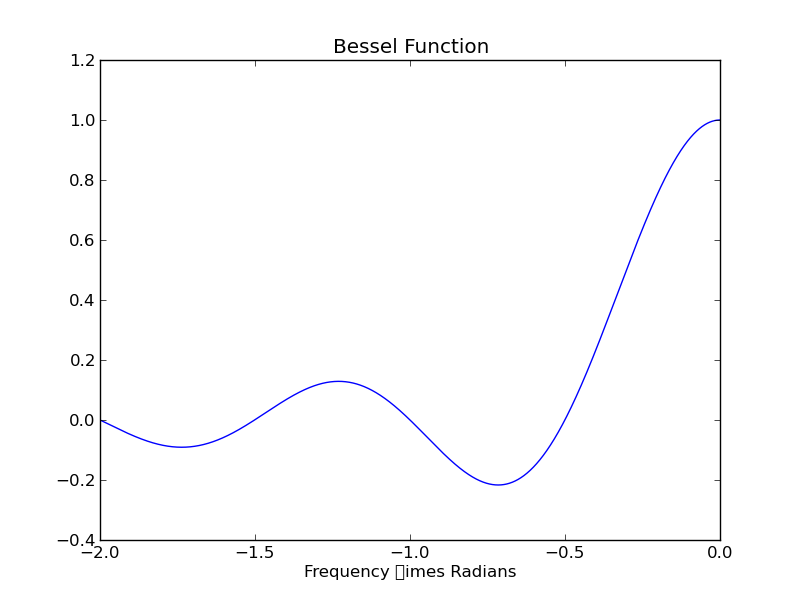
\includegraphics[scale=0.5]{img/sun/bessel.png}
    \caption{Ideal Bessel function}
    \label{fig:bessel_sun}
    \end{figure}

    Overlaying the Bessel function and a segment of the sun data shows a fairly
    obvious relationship. While the plot in Figure \ref{fig:compare_bessel} does
    not show the Bessel function as perfectly modeling the envelope of the
    measured sun data, it is roughly similar.

    \begin{figure}[h!]
    \centering
    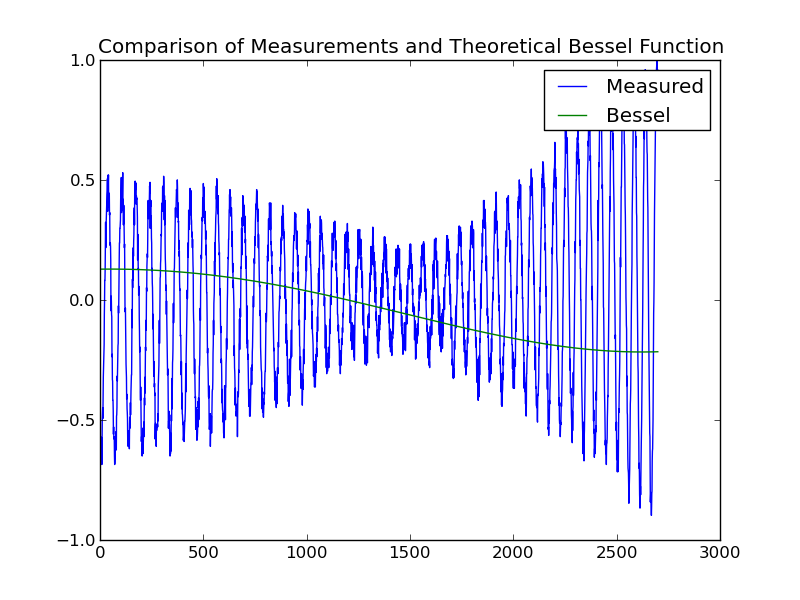
\includegraphics[scale=0.5]{img/sun/compare_bessel.png}
    \caption{Comparison of a segment of sun data and ideal Bessel function.}
    \label{fig:compare_bessel}
    \end{figure}

    In order to calculate the radius, and therefore diameter of the sun, we
    applied the same least squares techniques to the data as previously
    explained. After obtaining the least squares approximation, we found the
    envelope of the function by applying a simple method for AM demodulation
    (low pass filtering the absolute value of the signal). The minimum of the
    envelope allowed us to more precisely determine the points at which the
    measured data crossed 0. Figure \ref{fig:sun_analysis} shows the plots
    resulting from this analysis.

    \begin{figure}[h!]
    \centering
    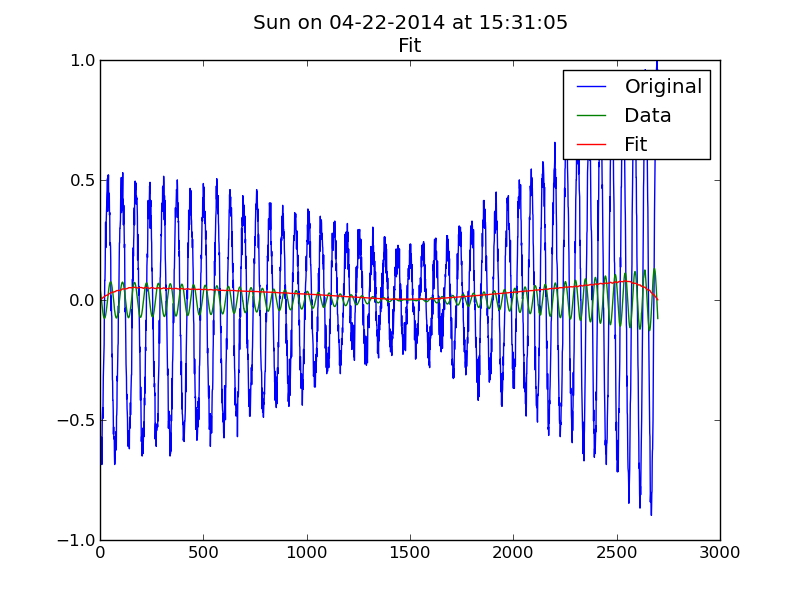
\includegraphics[scale=0.5]{img/sun/data_analysis.png}
    \caption{Least squares analysis to determine the local minimum of the
    sun data envelope.}
    \label{fig:sun_analysis}
    \end{figure}

    The residual shown in Figure \ref{fig:sun_residual} converges to a clear
    minimum unlike the previous analyses. The value of $\phi$ indicated by this
    plot appears to indicate a significant cable delay $\tau_c$ which is
    unlikely.

    \begin{figure}[h!]
    \centering
    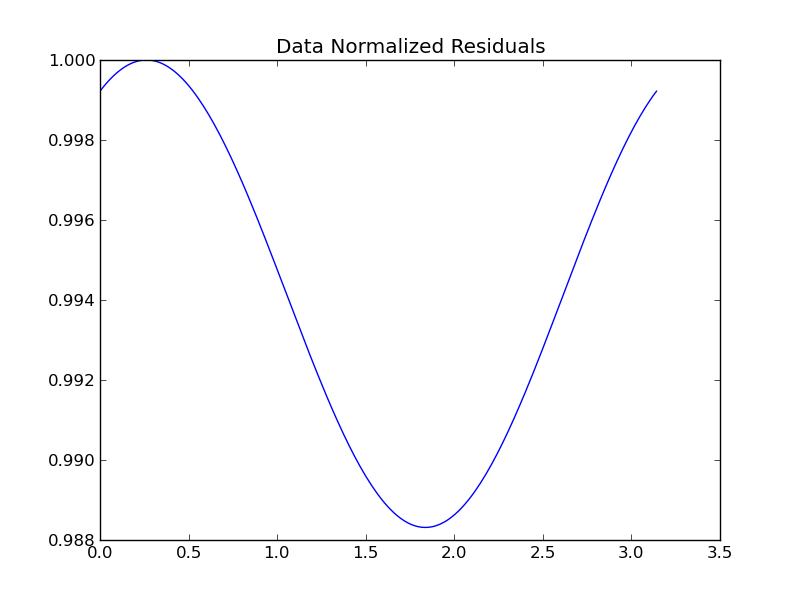
\includegraphics[scale=0.5]{img/sun/data_residual.png}
    \caption{Residuals from least squares fitting.}
    \label{fig:sun_residual}
    \end{figure}

    By using the hour angle $h_s$, declination $\delta$, and known baseline and
    wavelength values corresponding to the time of the detected zero crossing, we
    were able to solve for the fringe frequency $F_{f} = \left
    (\frac{B_{y}}{\lambda}\cos(\delta)\right )$. As previously explained for the
    second zero crossing (which we know this value corresponds to from Figure
    \ref{fig:compare_bessel}, we calculated the angular radius after making the
    appropriate unit conversions to be $\frac{2}{2F_f} = 0.2156^{\circ}$. The
    diameter is therefore $0.4312^{\circ}$.

    \FloatBarrier
\subsection{Moon}
    We applied the same techniques used for the sun to the data from the moon.
    The raw data from our observation of the moon on 4/6/2014 beginning at
    3:34:44 UTC is shown in Figure \ref{fig:raw_moon}.

    \begin{figure}[ht!]
    \centering
    \includegraphics[scale=0.5]{img/moon/raw.png}
    \caption{Raw data from the moon observation with the DC component subtracted
    such that the data is centered about 0.}
    \label{fig:raw_moon}
    \end{figure}

    The signal from the moon was significantly weaker considering the moon was
    only at approximately 30\% of its maximum illumination at the point on the
    date of the observation and the shape of the envelope is much less obvious.
    The peaks corresponding to the fringe frequency are also visually smaller in
    the plot of the spectrum shown in Figure \ref{fig:raw_moon}. We applied a
    band pass FIR filter with 256 coefficients centered about the observed peaks
    in the spectrum resulting in the plot shown in Figure
    \ref{fig:filtered_moon}. The filtered spectrum is also only a sub section of
    the data to remove the irregularities that occurred at roughly 1000 and
    12000 seconds (likely due to the re-pointing of the telescope).

    \begin{figure}[ht!]
    \centering
    \includegraphics[scale=0.5]{img/moon/filtered.png}
    \caption{Result of applying a band pass filter to isolate the frequencies of
    interest in a segment of moon data.}
    \label{fig:filtered_moon}
    \end{figure}

    After filtering the signal does appear to have an envelope roughly
    corresponding to the shape of a Bessel function. Because we began observing
    the source shortly after it had passed the meridian on that day, we compared
    it to the right half of a Bessel function shown in \ref{fig:bessel_moon}.

    \begin{figure}[h!]
    \centering
    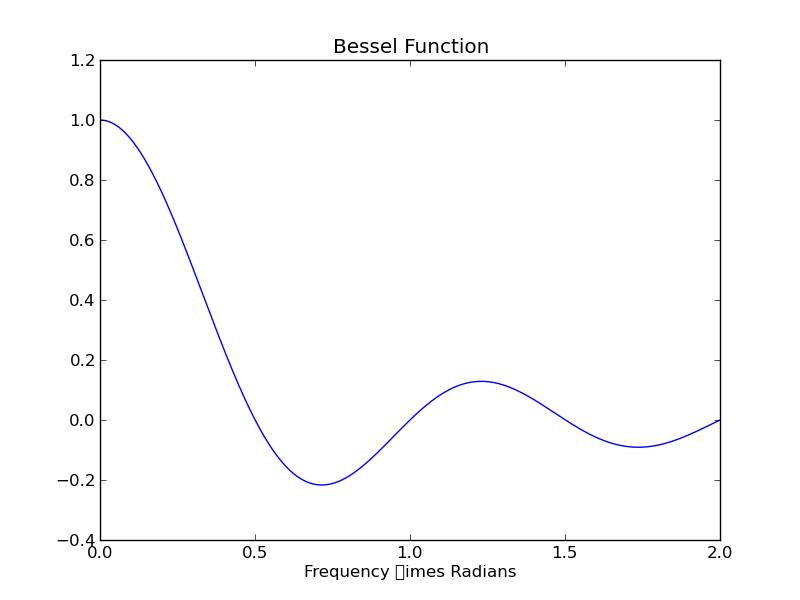
\includegraphics[scale=0.5]{img/moon/bessel.png}
    \caption{Ideal Bessel function}
    \label{fig:bessel_moon}
    \end{figure}

    As with the sun, we can identify the zero crossings corresponding to the
    Bessel function in our filtered data by overlaying the plots as shown in
    Figure \ref{fig:compare_bessel_moon}.

    \begin{figure}[ht!]
    \centering
    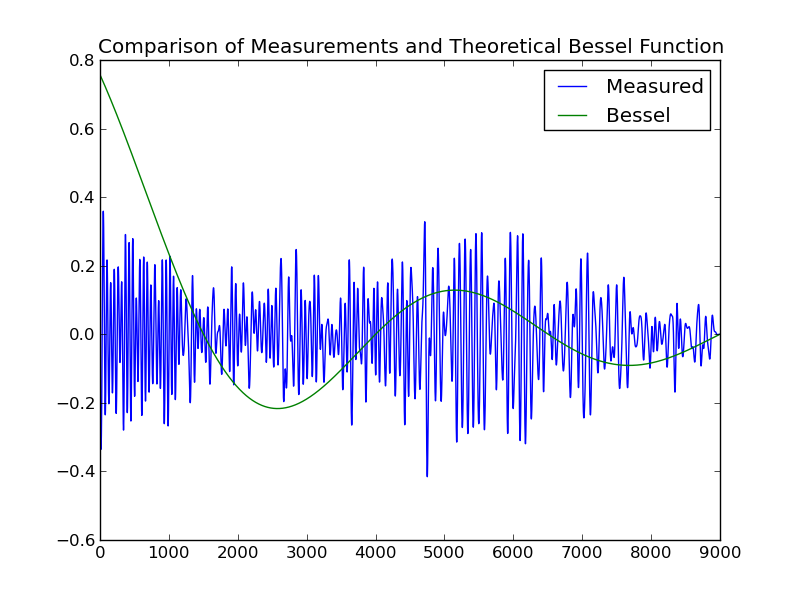
\includegraphics[scale=0.5]{img/moon/compare_bessel.png}
    \caption{Comparison of a segment of filtered moon data and ideal Bessel function.}
    \label{fig:compare_bessel_moon}
    \end{figure}

    We applied the same least squares techniques to determine the zero crossing
    of the filtered data \ref{fig:moon_analysis}. The residuals from this
    calculation are shown in Figure \ref{fig:moon_residual}. The results of the
    residual are similar to the sun which intuitively makes sense considering we
    had similar data and used the procedure. As in the case of the sun, the
    minimum of the residuals seems to indicate that $\phi$, corresponding to the
    cable delay $\tau_c$ which is still very significant unlikely.

    \begin{figure}[ht!]
    \centering
    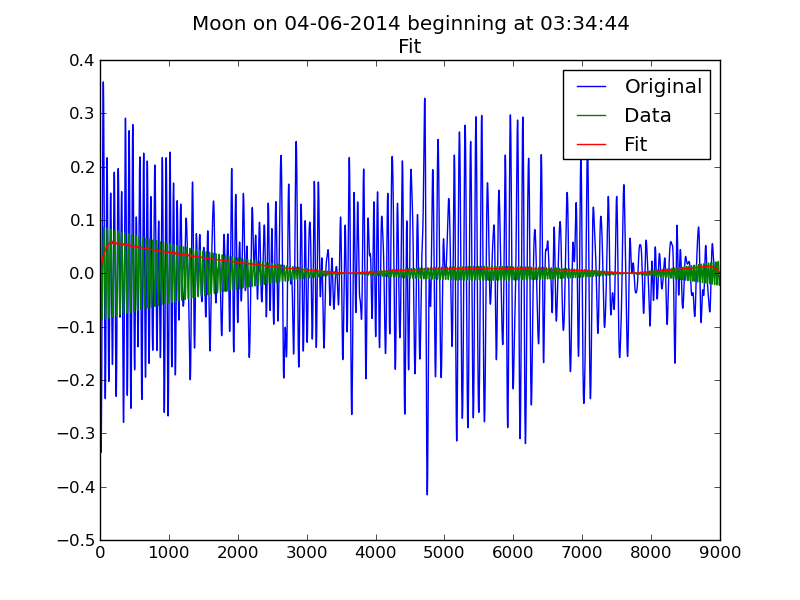
\includegraphics[scale=0.5]{img/moon/data_analysis.png}
    \caption{Least squares analysis to determine the local minimum of the
    moon data envelope.}
    \label{fig:moon_analysis}
    \end{figure}

    \begin{figure}[ht!]
    \centering
    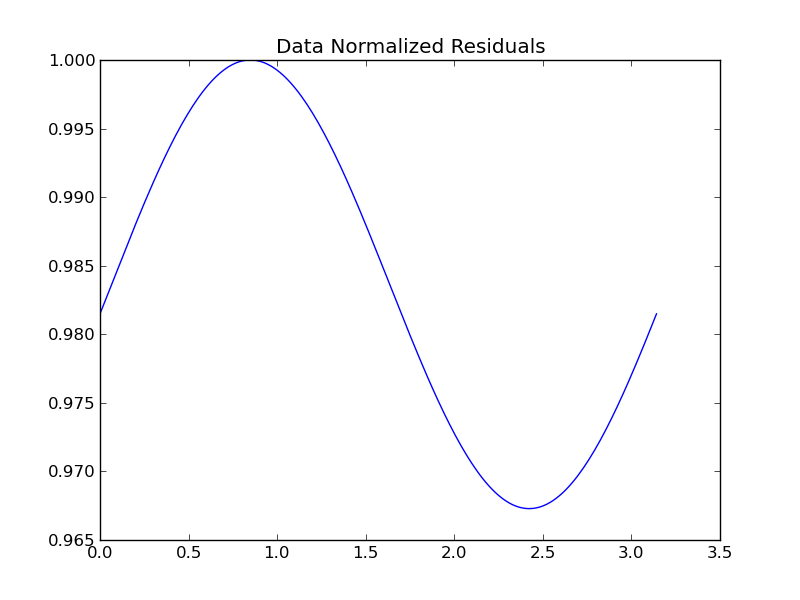
\includegraphics[scale=0.5]{img/moon/data_residual.png}
    \caption{Residuals from least squares fitting.}
    \label{fig:moon_residual}
    \end{figure}

    We used the same equations to compute the radius of the moon to be
    $R=0.17422^{\circ}$. The diameter is therefore $D = 0.34844^{\circ}$. This value is
    significantly smaller than the known diameter of the moon $D = 0.4922^{\circ}$,
    however as shown the data was relatively noisy and our filtering may have
    affected frequencies of interest.


    \FloatBarrier
%=======================================================================================
\section{Conclusion}
This lab experiment was a valuable exercise in the applications of signal
processing and data analysis. As expected, the data we recorded, despite the
precautions we took to minimize error were far from ideal. We were able to
compensate for this and achieve reasonable results by filtering out noise and
using least squares to develop approximations of our data.
\\
\\
Code for the analysis and observation are not included in the body of this
document but are both available online at: https://github.com/viyer/astro121.
All original data and log files from the observations are available here as
well.

%   \bibliographystyle{plain}
%   \bibliography{references}
\end{document}
